\section{Results}
\label{sec:results}

We report results in four parts: (\secref{sec:heatmaps}) the main depth$\times$width heatmap grid, (\secref{sec:hypotheses}) hypothesis tests H1--H5, (\secref{sec:metric_agreement}) cross-metric agreement, and (\secref{sec:ablations}) the rich-vs-lazy, shuffled-label, and dominant-datapoint ablations.

\subsection{Cross-layer CKA heatmaps}
\label{sec:heatmaps}

\Figref{fig:heatmaps} shows the depth$\times$width grid of mean cross-layer \ckam heatmaps on \cifar and \mnist. Three regimes are visible at a glance.

\begin{itemize}[leftmargin=*,itemsep=0pt,topsep=0pt]
    \item \textbf{Shallow ($d\!=\!4$)}: every layer is distinguishable. No block structure. Mean off-diagonal CKA ranges from $0.70$ at $w\!=\!128$ down to $0.50$ at $w\!=\!2048$ on \cifar.
    \item \textbf{Intermediate ($d\!=\!8$)}: a mid-network block starts to form; the final hidden layer remains distinct.
    \item \textbf{Deep ($d\!=\!16$)}: layers $2\!-\!14$ collapse into a single block with CKA $\gtrsim\!0.9$; only the input- and output-proximal layers stay distinct.
\end{itemize}

The block-structure phenomenon---previously documented only for CNNs, ResNets~\citep{nguyen2021wide,nguyen2022origins}, and transformers~\citep{brown2023dissimilarity}---is cleanly reproducible in pure ReLU MLPs at $d\!=\!16$.

\begin{figure}[t]
    \centering
    \begin{subfigure}[b]{0.48\textwidth}
        \centering
        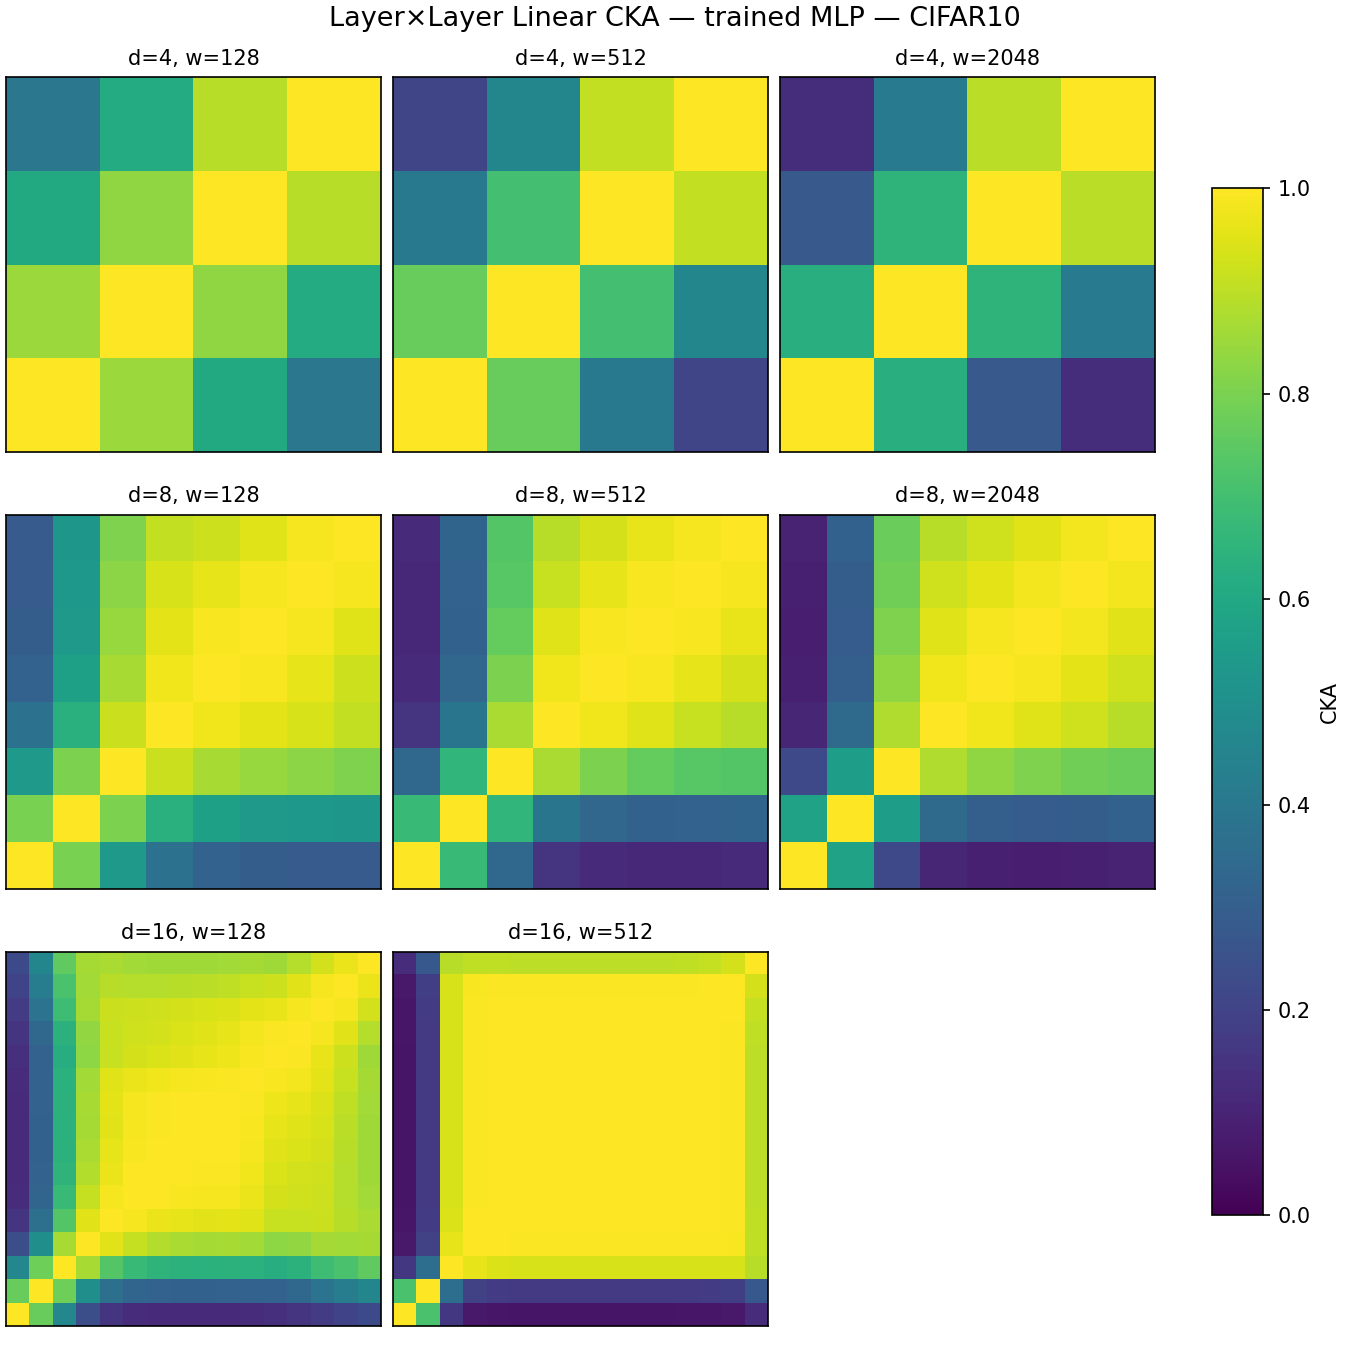
\includegraphics[width=\linewidth]{figures/cka_heatmap_grid_cifar10.png}
        \caption{\cifar}
        \label{fig:heatmaps_cifar}
    \end{subfigure}
    \begin{subfigure}[b]{0.48\textwidth}
        \centering
        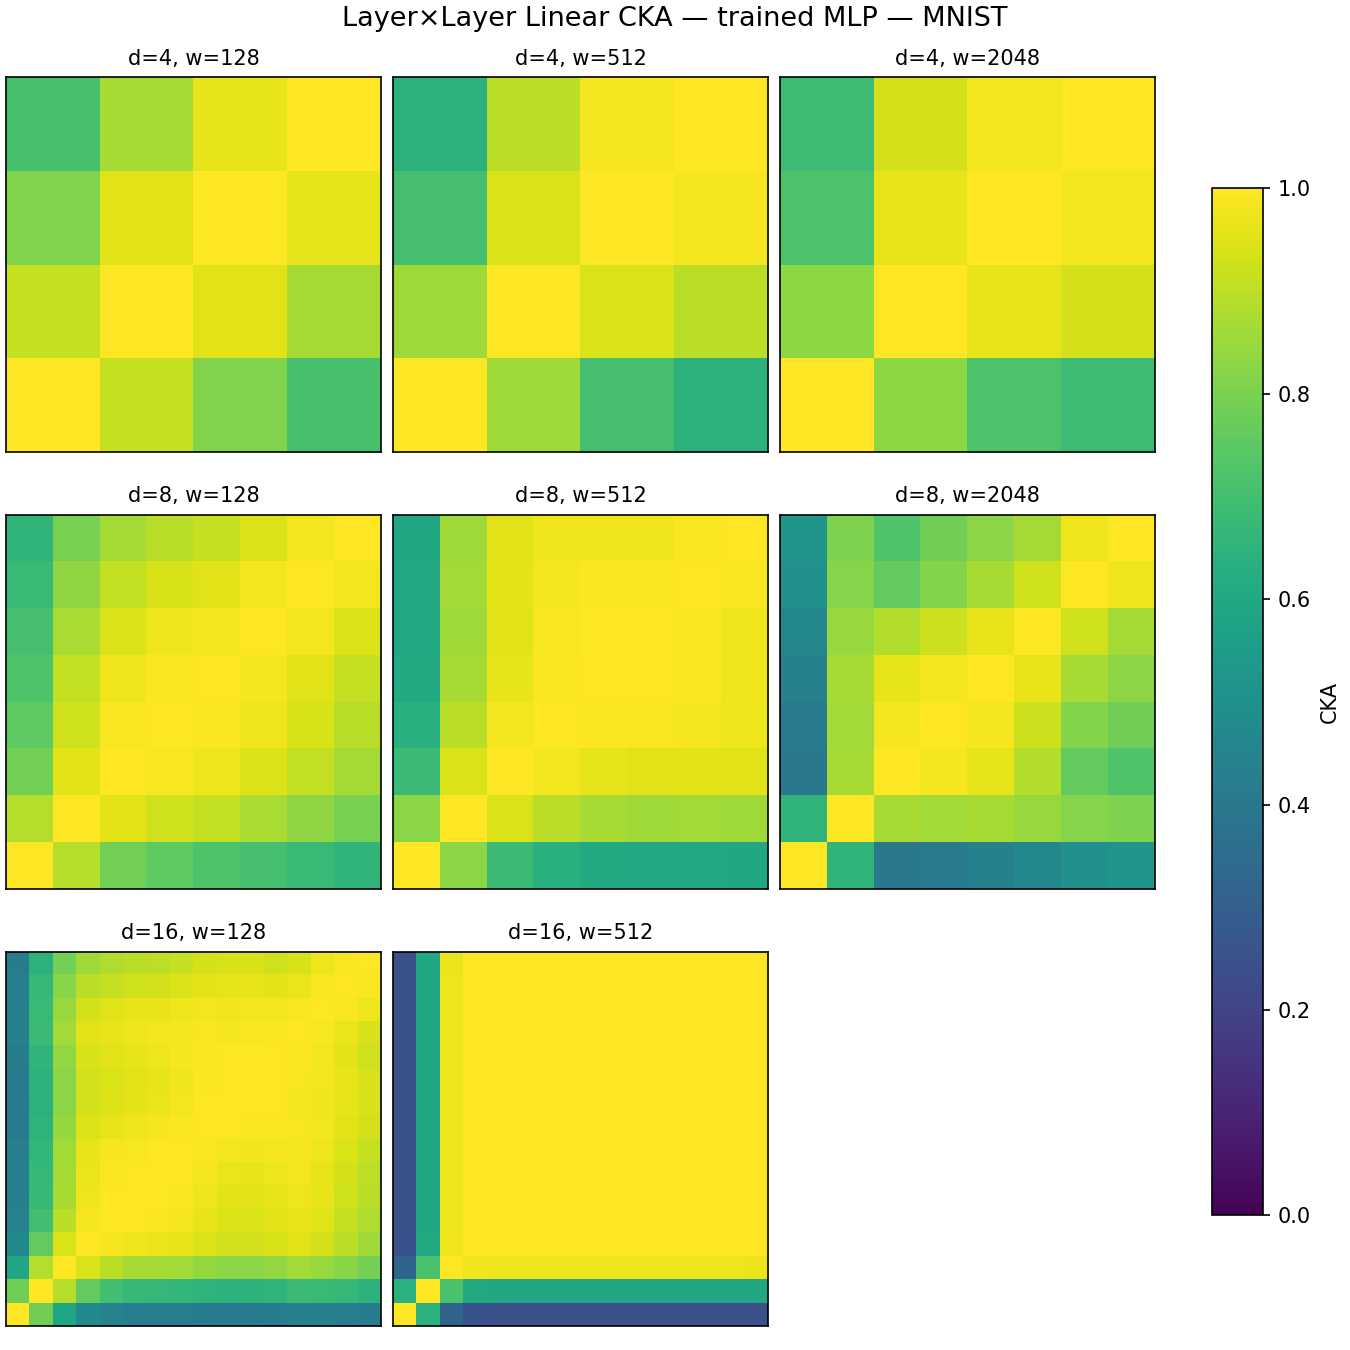
\includegraphics[width=\linewidth]{figures/cka_heatmap_grid_mnist.png}
        \caption{\mnist}
        \label{fig:heatmaps_mnist}
    \end{subfigure}
    \caption{Mean cross-layer \ckam (over three seeds) for every $(d,w)$ in the sweep. Rows $=$ depth $\{4,8,16\}$, columns $=$ width $\{128,512,2048\}$. Deep networks ($d\!=\!16$, top row) develop a contiguous bright block that covers almost the entire interior. Shallow networks ($d\!=\!4$, bottom row) show a smooth gradient instead.}
    \label{fig:heatmaps}
\end{figure}

\Figref{fig:cka_vs_k} summarizes the same information as a 1-D decay curve: mean \ckam between layers $L$ and $L\!+\!k$ as a function of the gap $k$. The decay is monotone for all depths, but far shallower for the $d\!=\!16$ MLP---at $k\!=\!10$, \ckam is still $\approx\!0.6$ because of the large central block.

\begin{figure}[t]
    \centering
    \begin{subfigure}[b]{0.48\textwidth}
        \centering
        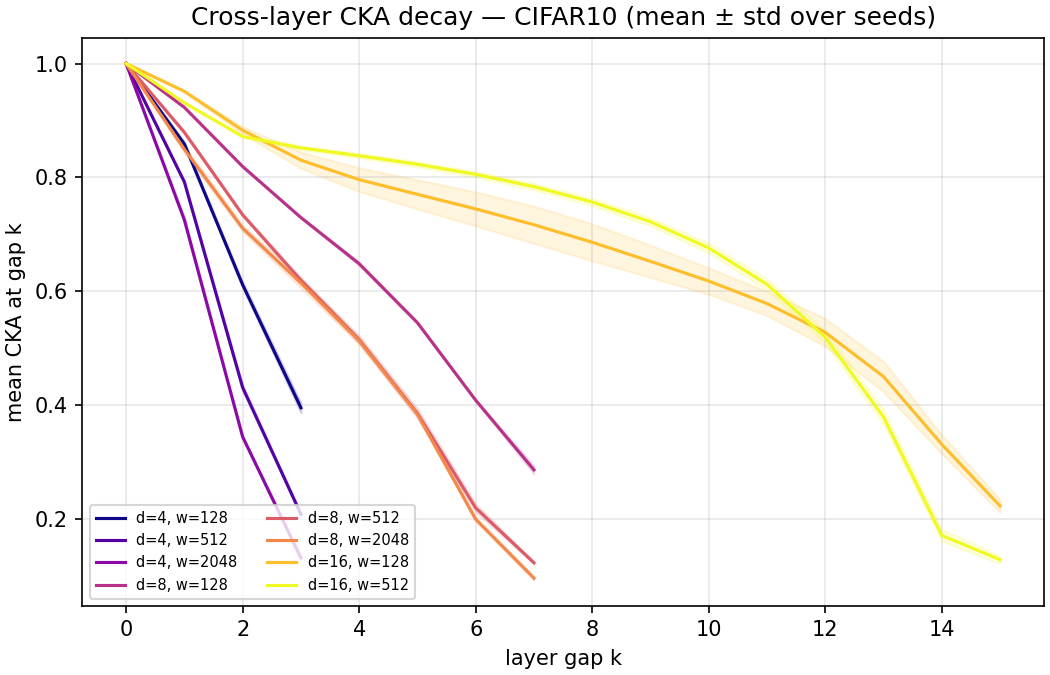
\includegraphics[width=\linewidth]{figures/cka_vs_k_cifar10.png}
        \caption{\cifar}
    \end{subfigure}
    \begin{subfigure}[b]{0.48\textwidth}
        \centering
        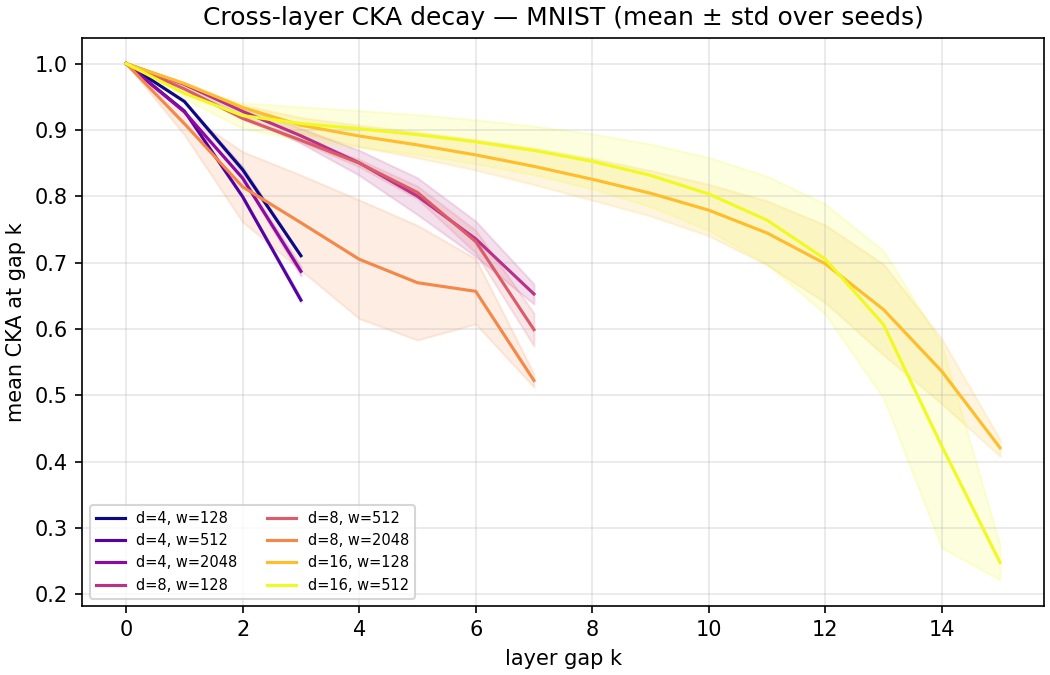
\includegraphics[width=\linewidth]{figures/cka_vs_k_mnist.png}
        \caption{\mnist}
    \end{subfigure}
    \caption{Mean \ckam between layers $L$ and $L\!+\!k$ as a function of the gap $k$. Deeper MLPs decay more slowly because of the central block; shallow MLPs show sharp drops.}
    \label{fig:cka_vs_k}
\end{figure}

\subsection{Hypothesis tests}
\label{sec:hypotheses}

\Tabref{tab:hypotheses} summarizes the six statistical tests derived from \texttt{results/hypothesis\_tests.json}. H1 (adjacent layers are more similar than far-apart layers) is confirmed with $p\!\ll\!10^{-3}$ on both datasets. H5 (rich-regime MLPs have lower cross-layer CKA) is confirmed on \cifar ($\rho\!=\!-0.54$, $p\!=\!0.003$). The most striking finding is H2: at $d\!\leq\!8$, width and CKA are \emph{strongly negatively correlated} on \cifar ($\rho\!=\!-0.95$), meaning wider MLPs produce \emph{less} similar layers---the opposite of the \citet{kornblith2019similarity} CNN finding. At $d\!=\!16$ the correlation flips sign (and loses significance), indicating a regime transition.

\begin{table}[t]
    \centering
    \caption{Hypothesis tests on the main sweep. H2 reveals a sign reversal with depth: negative correlation at $d\!\leq\!8$ (wider $\Rightarrow$ less similar), non-significant at $d\!=\!16$ once block structure dominates.}
    \label{tab:hypotheses}
    \begin{tabular}{@{}lllll@{}}
        \toprule
        \textbf{Test} & \textbf{Dataset} & \textbf{Statistic} & \textbf{$p$-value} & \textbf{$N$} \\
        \midrule
        H1 adjacent vs.\ far-layer CKA & \cifar & $t\!=\!14.3$ (adj 0.864, far 0.460) & $6.6\times 10^{-13}$ & 24 \\
        H1 adjacent vs.\ far-layer CKA & \mnist & $t\!=\!14.2$ (adj 0.947, far 0.758) & $1.5\times 10^{-12}$ & 23 \\
        H2 width $\leftrightarrow$ CKA ($d\!=\!4$) & \cifar & $\rho\!=\!-0.949$ & $9.6\times 10^{-5}$ & 9 \\
        H2 width $\leftrightarrow$ CKA ($d\!=\!8$) & \cifar & $\rho\!=\!-0.949$ & $9.6\times 10^{-5}$ & 9 \\
        H2 width $\leftrightarrow$ CKA ($d\!=\!16$) & \cifar & $\rho\!=\!+0.488$ & $0.33$ & 6 \\
        H2 width $\leftrightarrow$ CKA ($d\!=\!8$) & \mnist & $\rho\!=\!-0.794$ & $0.019$ & 8 \\
        H5 $\|\Delta\theta\|/\|\theta_0\| \leftrightarrow$ CKA & \cifar & $\rho\!=\!-0.540$ & $0.003$ & 28 \\
        H5 $\|\Delta\theta\|/\|\theta_0\| \leftrightarrow$ CKA & \mnist & $\rho\!=\!-0.299$ & $0.17$ & 23 \\
        \bottomrule
    \end{tabular}
\end{table}

\subsection{Cross-metric agreement}
\label{sec:metric_agreement}

\Figref{fig:metric_agreement} shows the rank correlations across metrics on \cifar. \procrustes and \ckam track each other at $\rho\!=\!0.98$. Sample-wise cosine similarity is weaker in absolute value but agrees on the ranking of layer pairs ($\rho\!=\!0.72$). This addresses the \citet{davari2022reliability} concern: no metric is the outlier, and all three point to the same cross-layer structure.

\begin{figure}[t]
    \centering
    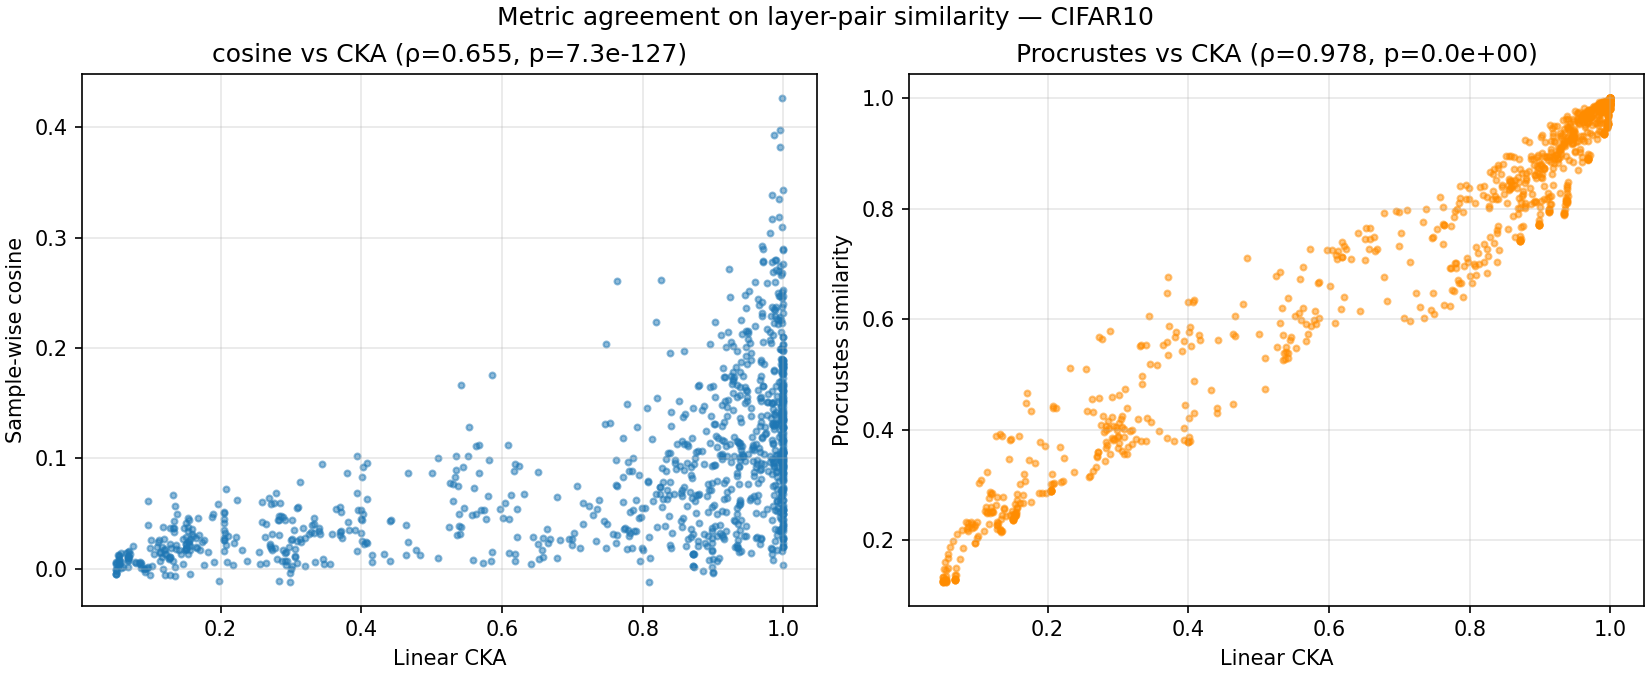
\includegraphics[width=0.75\linewidth]{figures/metric_agreement_cifar10.png}
    \caption{Pairwise agreement between \ckam, \procrustes, and \samplecos on \cifar. Each point is one layer-pair in the sweep. \procrustes and \ckam are in essentially linear agreement; cosine is systematically lower but rank-consistent.}
    \label{fig:metric_agreement}
\end{figure}

\subsection{Training changes cross-layer CKA}
\label{sec:training_vs_init}

\Figref{fig:init_vs_trained} plots mean off-diagonal CKA of the trained network against that of the same network at initialization. For shallow MLPs ($d\!=\!4$, purple) training decisively lowers CKA---layers differentiate from each other during learning. For deep MLPs ($d\!=\!16$, yellow) training approximately preserves the initial CKA profile. The depth-dependent similarity structure is thus a \emph{learning} phenomenon, not an initialization artifact.

\begin{figure}[t]
    \centering
    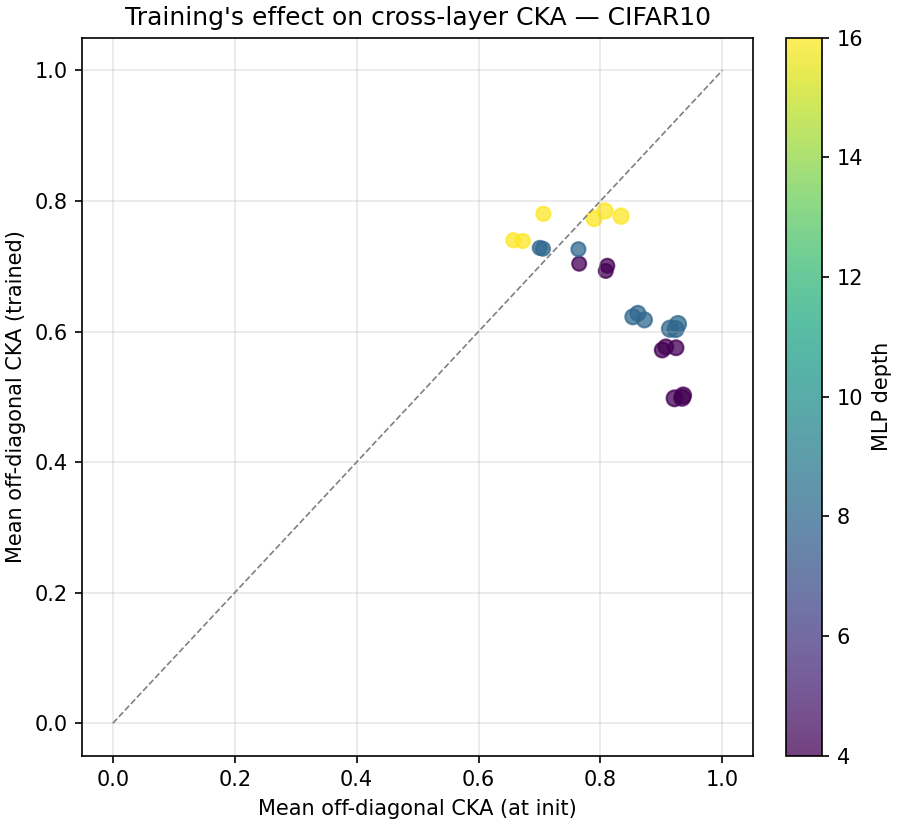
\includegraphics[width=0.55\linewidth]{figures/init_vs_trained_cka_cifar10.png}
    \caption{Mean off-diagonal \ckam at initialization (x-axis) vs.\ after training (y-axis) on \cifar. Points below the diagonal indicate that training \emph{reduced} cross-layer similarity. Color encodes depth.}
    \label{fig:init_vs_trained}
\end{figure}

\subsection{Per-layer linear probes}
\label{sec:probes}

\Figref{fig:probe} shows probe accuracy as a function of layer index for every $(d,w)$. Accuracy rises sharply in the first one to two hidden layers, then plateaus. For $d\!=\!16$, the plateau begins remarkably early and is nearly flat through the block---consistent with the \ckam block-structure story: if layers 2--14 are near-identical, their linear probes \emph{must} be near-identical.

\begin{figure}[t]
    \centering
    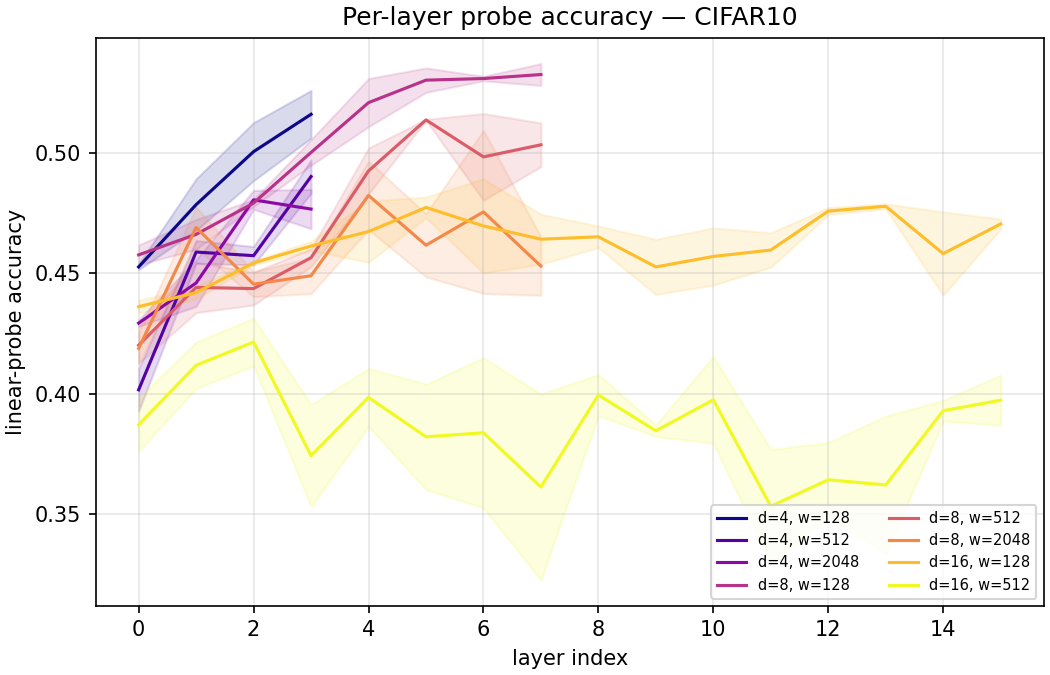
\includegraphics[width=0.75\linewidth]{figures/probe_acc_curves_cifar10.png}
    \caption{Per-layer linear-probe accuracy on \cifar, one curve per $(d,w)$. Deep MLPs ($d\!=\!16$) plateau early, mirroring the block structure seen in the \ckam heatmaps.}
    \label{fig:probe}
\end{figure}

\subsection{Ablations}
\label{sec:ablations}

\para{Rich vs.\ lazy.} Sweeping the initialization scale $\alpha$ on \mlp{8}{512}, \cifar (\Tabref{tab:rich_lazy}) confirms \citet{tong2025richness}'s prediction. The lazy extreme ($\alpha\!=\!4.0$) gives the highest cross-layer CKA (0.76) but the \emph{lowest} test accuracy (0.40)---representations are similar because the network never moved far from initialization. The rich extreme ($\alpha\!=\!0.25$) gives the lowest CKA (0.50) and good accuracy. \Figref{fig:rich_lazy} visualizes the full trajectory.

\begin{table}[t]
    \centering
    \caption{Rich-vs-lazy ablation on \mlp{8}{512}, \cifar, seed 0. Lazy MLPs (small $\|\Delta\theta\|/\|\theta_0\|$) have nearly-identical layers but fail to learn.}
    \label{tab:rich_lazy}
    \begin{tabular}{@{}rrrr@{}}
        \toprule
        init-scale $\alpha$ & test acc & $\|\Delta\theta\|/\|\theta_0\|$ & mean off-diag \ckam \\
        \midrule
        0.25 & 0.521 & 4.83 & 0.498 \\
        0.50 & 0.527 & 2.34 & 0.500 \\
        1.00 & 0.532 & 1.18 & 0.628 \\
        2.00 & 0.536 & 0.56 & 0.640 \\
        4.00 & 0.398 & 0.09 & \textbf{0.760} \\
        \bottomrule
    \end{tabular}
\end{table}

\begin{figure}[t]
    \centering
    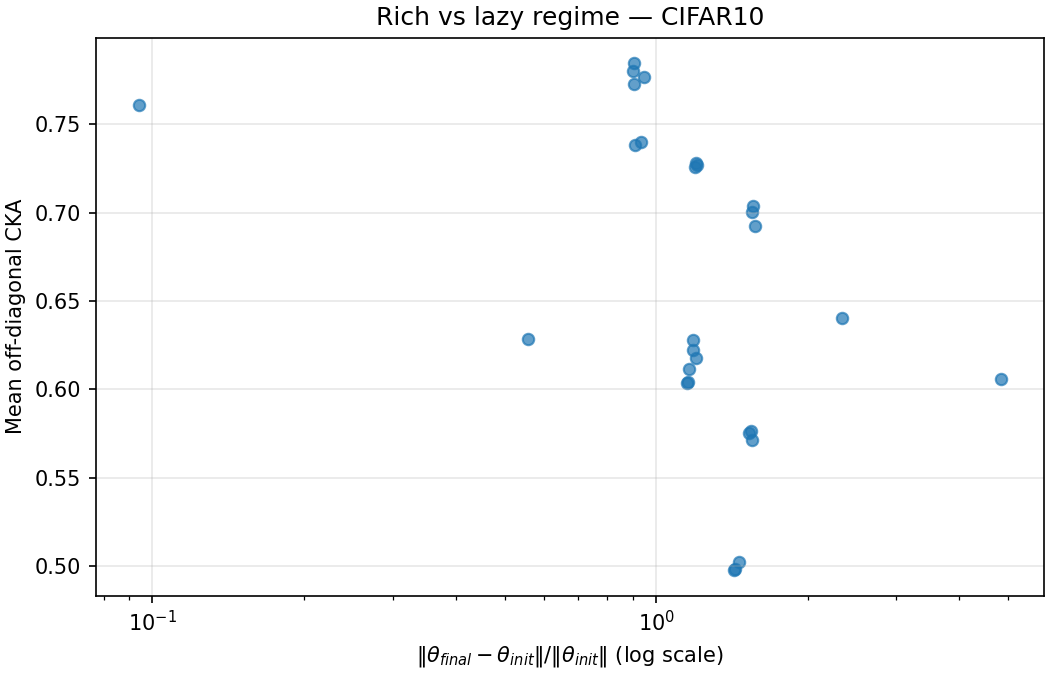
\includegraphics[width=0.6\linewidth]{figures/rich_lazy_cifar10.png}
    \caption{Rich-vs-lazy: increasing initialization scale (\emph{x-axis, inverted-rich-to-lazy}) pulls trained MLPs closer to their initialization and raises mean off-diagonal \ckam. Test accuracy is non-monotonic---high CKA in the lazy regime reflects failure to learn, not successful representation sharing.}
    \label{fig:rich_lazy}
\end{figure}

\para{Shuffled-label control.} Training \mlp{8}{512} on \cifar with labels permuted uniformly at random yields mean off-diagonal CKA $= 0.541$---only $0.087$ below the true-label run (0.628)---while test accuracy collapses to 0.09. The cross-layer similarity structure is therefore driven more by architecture and optimization than by task-relevant signal.

\para{Dominant-datapoint ablation.} For the same \mlp{8}{512} reference, excluding the top-decile highest-activation-norm probe samples reduces mean off-diagonal \ckam by $\Delta\!=\!-0.011$ (from 0.628 to 0.617). For comparison, \citet{nguyen2022origins} reported $\Delta \approx\!-0.15$ for CNN block structure. The dominant-datapoint mechanism is present in MLPs but an order of magnitude weaker than in CNNs, suggesting the block structure we observe at $d\!=\!16$ has a different proximate cause---likely the identity-channel behavior of deep ReLU stacks rather than a small subset of trivial-image-statistics examples.
